%*****************************************
\chapter{Introducci\'on}\label{ch:antecedentes}
%*****************************************

Este capítulo inicia presentando una vía de señalización relacionada con la motilidad del espermatozoide de erizo de mar. Posteriormente presenta un modelo discreto para dicha vía de señalización, señalando sus alcances y limitaciones. Seguidamente se muestra un formalismo semicontinuo que promete llevar las comparaciones entre modelo y experimento a un nivel más cuantitativo, así como algunos detalles relevantes para la transformación de un modelo discreto en el formalismo semicontinuo antes mencionado.

\section{La v\'ia de se\~nalizaci\'on de speract}\label{sec:spSigNet}

La fertilización es un proceso crucial para la transmisión de la vida, que requiere el encuentro y fusión de los gametos. Para que este encuentro tenga lugar, el espermatozoide debe valerse de una intrincada maquinaria en su flagelo que le permita nadar en busca del óvulo. En algunas especies, el óvulo secreta una sustancia quimioatrayente que guía al esperma hacia él. En el caso particular del erizo de mar, esta sustancia es un decapéptido llamado \emph{speract}, \citeauthor{SUZUKI:1995gp} \citep{SUZUKI:1995gp}, \citeauthor{Hansbrough:1981vk} \citep{Hansbrough:1981vk}, el cual se une a un receptor específico en la membrana del flagelo del espermatozoide. La unión de speract con su receptor activa una red de señalización que produce oscilaciones en la concentración interna de algunos iones, de los cuales el principal es el \ac{ca} \citeauthor{Darszon2008} \citep{Darszon2008}. 

La vía de señalización inducida por speract provoca la apertura de distintos canales que hiperpolarizan la membrana, es decir, que disminuyen drásticamente la polaridad de la membrana \citeauthor{Kaupp:2008gv} \citep{Kaupp:2008gv}. A su vez, esta hiperpolarización cancela la desactivación de canales regulados por voltaje, que al abrirse despolarizan la membrana \citeauthor{Strunker:2006tk} \citep{Strunker:2006tk}, \citeauthor{GranadosGonzalez:2005ia} \citep{GranadosGonzalez:2005ia}. La despolarización se refiere al proceso de regresar la polaridad de la membrana a sus niveles basales. El proceso repetido de hiper y despolarización se ha relacionado con cambios transitorios en la concentración de calcio intracelular que a su vez han sido relacionados con cambios en la curvatura del flagelo del espermatozoide que resultan en modificaciones abruptas de su trayectoria \citeauthor{Darszon2008} \citep{Darszon2008}. Estos cambios de trayectoria son una parte esencial para la motilidad y reorientación del esperma. De ahí la importancia de entender los mecanismos bioquímicos que la generan. 

Las oscilaciones de \ac{calintra} se caracterizan por presentar un incremento sostenido \emph{(tónico)} y fluctuaciones superimpuestas \emph{(supratónico)}. Las oscilaciones tónicas corresponden al incremento sostenido en \ac{calintra}. Este tipo de oscilaciones de \ac{calintra} se presentan tanto en la cabeza como en el flagelo del espermatozoide tras la activación de la vía de señalización mediante la adición de speract al medio. La figura \ref{fig:fluorescencia} muestra una medición experimental de las oscilaciones, obtenida al añadir un marcador fluorescente al \ac{ca} y liberar moléculas de \ac{SR} en el medio. Los detalles experimentales se describen a profundidad en \citeauthor{Darszon2008} \citep{Darszon2008} y \citeauthor{Wood2007} \citep{Wood2007}. En la figura, la serie en rojo corresponde a la concentración de \ac{calintra} en la cabeza, mientras que los datos en color negro corresponden a la concentración de \ac{calintra} en el flagelo, ambas medidas a través del tiempo. En la serie correspondiente al flagelo, se observa la componente tónica en el incremento de la fluorescencia al rededor de los 3 ó 4 segundos, mismo que se mantiene a lo largo de la medición. Nótese que este comportamiento también se observa en la cabeza (serie roja). Sin embargo, el comportamiento del \ac{calintra} es distinto en el flagelo que en la cabeza del espermatozoide, puesto que adicionalmente se observan las oscilaciones supratónicas, es decir, aquellas que parecen superpuestas o "montadas" a lo largo de toda la serie. Estas últimas oscilaciones presentan poca amplitud al principio de la medición, es decir, previo a la adición de \ac{SR}, e incrementan su amplitud tras la adición de \ac{SR} y activación de la vía de señalización. La barra de color magenta en la parte inferior, que inicia poco después de la marca de los 2 segundos muestra el momento en el que el \ac{SR} comienza a estimular la vía de señalización y el tiempo en la que ésta se mantiene activa.


\begin{figure}[hbt]
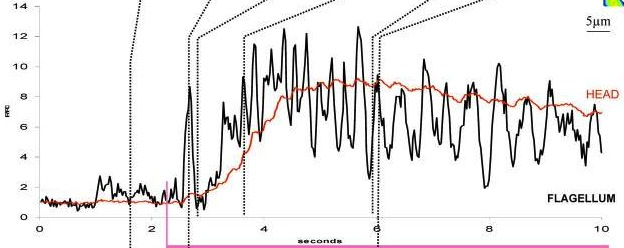
\includegraphics[width=0.9\linewidth]{gfx/maderaSperact}
\caption[Medición experimental de calcio intracelular]{Medición experimental de fluorescencia de calcio intracelular en espermatozoides. Se muestran mediciones para la cabeza (rojo) y el flagelo (negro) del espermatozoide. %Las oscilaciones tónicas corresponden al incremento sostenido en la concentración de \ac{ca}, y tienen una forma sigmoidal. Este tipo de oscilaciones se presentan tanto en la cabeza como en el flagelo del espermatozoide. En la figura, la serie en rojo corresponde a la concentración de \ac{ca} en la cabeza, mientras que los datos en color negro corresponden a la concentración de \ac{ca} en el flagelo. Las oscilaciones supratónicas se observan solamente en el flagelo y se distinguen por ser las fluctuaciones que parecen "montarse"\ sobre la curva con forma sigmoidal. La barra de color rojo en la parte inferior, que inicia poco después de la marca de los 2 segundos muestra el momento en el que el speract comienza a estimular la vía de señalización y el tiempo en la que ésta se mantiene activa.
Figura modificada tomada de \citeauthor{Wood:2003p4517} \citep{Wood:2003p4517}.}\label{fig:fluorescencia}
\end{figure}

La figura \ref{fig:erizobBioquimica} \textsc{A} muestra el diagrama de la vía de señalización de speract, que consta del \ac{SR}, así como de varios canales e intercambiadores íonicos, entre otros componentes. La parte superior representa el exterior del flagelo, la parte gris es la membrana celular y debajo de esta se encuentra el interior de la célula. En esa misma figura, el apartado \textsc{B} muestra de manera esquemática los eventos de la vía de señalización, mismos que se detallan a continuación.

La vía de señalización inicia con la unión de speract a su receptor \acs{SR} \citeauthor{Darszon2008} \citep{Darszon2008}, que interacciona con una \ac{gc} \citeauthor{Garbers:1976wy} \citep{Garbers:1976wy}, la cual a su vez produce \ac{cGMP}. El aumento en la concentración de \ac{cGMP} abre el \ac{kcng} \citeauthor{Galindo:2007bx} \citep{Galindo:2007bx}. La apertura de \ac{kcng} resulta en la hiperpolarización del \ac{v} \citeauthor{Strunker:2006tk} \citep{Strunker:2006tk}. Como consecuencia de la hiperpolarización suceden cuatro eventos importantes:
\begin{enumerate}
\item se activa un \ac{nce} que disminuye los niveles de \ac{calintra} \citeauthor{Nishigaki:2004p4516} \citep{Nishigaki:2004p4516} 
\item se activa un \ac{nhe} que incrementa el \ac{phi} \citeauthor{Lee:1986vs} \citep{Lee:1986vs} \citeauthor{Wang:2003ke} \citep{Wang:2003ke}, \citeauthor{Su:2002fk} \citep{Su:2002fk}, \citeauthor{Rodriguez:2003do} \citep{Rodriguez:2003do}
\item se activa un \ac{hcn} \citeauthor{Nishigaki:2004p4516} \citep{Nishigaki:2004p4516}, \citeauthor{Rodriguez:2003do} \citep{Rodriguez:2003do}, \citeauthor{Gauss:1998de} \citep{Gauss:1998de}, \citeauthor{Galindo:2005wf} \citep{Galindo:2005wf}
\item finalmente, la sustracción de la inactivación del \ac{hva} y el \ac{lva} \citeauthor{Strunker:2006tk} \citep{Strunker:2006tk}, \citeauthor{GranadosGonzalez:2005ia} \citep{GranadosGonzalez:2005ia}, \citeauthor{Wood:2003p4517} \citep{Wood:2003p4517}, \citeauthor{Wood:2005gg} \citep{Wood:2005gg}, \citeauthor{Darszon:2005tb} \cite{Darszon:2005tb}, \citeauthor{PerezReyes:2003bw} \citep{PerezReyes:2003bw}
\end{enumerate}

%\graffito{La figura \ref{fig:erizobBioquimica} \textsc{B} muestra los eventos de la vía de señalización usando una notación estándar en los esquemas de regulación biológica: los arcos o aristas dirigidas de color negro que acaban en punta representan activación o regulación positiva, mientras que los arcos rojos que acaban en una línea llana representan inhibición o regulación negativa.}

\begin{figure}[hbt]
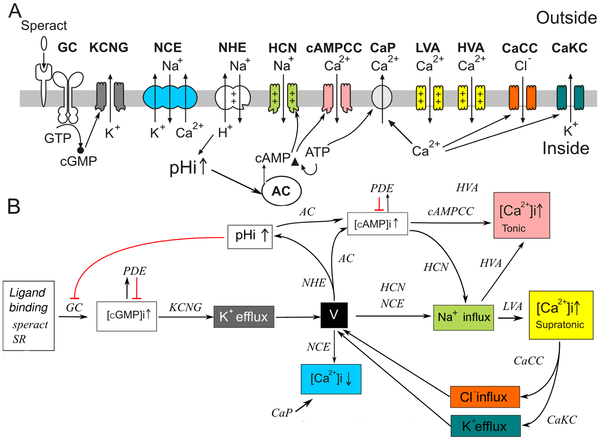
\includegraphics[width=0.9\linewidth]{gfx/redErizoBioquimica}
\caption[Red de se\~nalizaci\'on]{Red de se\~nalizaci\'on \citeauthor{Espinal2011} \citep{Espinal2011}.\\
A) Componentes principales involucrados en la vía de señálización de speract. La unión de speract a su receptor en la membrana del flagelo dispara la cascada que produce cambios en \ac{calintra} a través de la entrada y salida de iones a través de intercambiadores, bombas y canales.
\\
B) Esquema de eventos producidos por la vía de señalización. En este esquema, se muestran los eventos de la vía de señalización usando una notación estándar en los esquemas de regulación biológica: los arcos o aristas dirigidas de color negro que acaban en punta representan activación o regulación positiva, mientras que los arcos rojos que acaban en una línea llana representan inhibición o regulación negativa.}\label{fig:erizobBioquimica}
\end{figure}

El incremento del \ac{phi} disminuye la actividad de \ac{gc} a la vez que activa una \ac{AC}, con la consecuente producción de \ac{cAMP}, \citeauthor{Nishigaki:2004p4516} \citep{Nishigaki:2004p4516}, \citeauthor{Cook:1993ul} \citep{Cook:1993ul}, \citeauthor{Beltran:1996fd} \citep{Beltran:1996fd}. Este último estimula un \ac{cAMPCC} y el canal \ac{hcn} previamente activado, lo cual tiende a repolarizar el potencial de membrana \acs{v} \citeauthor{Strunker:2006tk} \citep{Strunker:2006tk}, \citeauthor{Kaupp:2003p4518} \citep{Kaupp:2003p4518}, \citeauthor{Nishigaki:2004p4516} \citep{Nishigaki:2004p4516}, \citeauthor{Rodriguez:2003do} \citep{Rodriguez:2003do}, \citeauthor{Gauss:1998de} \citep{Gauss:1998de}. Esta repolarización abre los canales \ac{hva} y \ac{lva} causando una despolarización y un incremento del \ac{calintra}, \citeauthor{Strunker:2006tk} \citep{Strunker:2006tk}, \citeauthor{GranadosGonzalez:2005ia} \citep{GranadosGonzalez:2005ia}, \citeauthor{Kaupp:2003p4518} \citep{Kaupp:2003p4518},\citeauthor{Bohmer:2005ik} \citep{Bohmer:2005ik}, \citeauthor{Wood:2003p4517} \citep{Wood:2003p4517}, \citeauthor{Nishigaki:2004p4516} \citep{Nishigaki:2004p4516}, \citeauthor{Wood:2005gg} \citep{Wood:2005gg}. Finalmente, la vía de señalización se inicia de nuevo, posiblemente a través de un \ac{cacc} y un \ac{cakc} \citeauthor{Wood:2003p4517} \citep{Wood:2003p4517}, \citeauthor{Wood2007} \citep{Wood2007}, \citeauthor{Greenwood:2007hg} \citep{Greenwood:2007hg}, que se abren cuando la concentración de \ac{calintra} es alta. Los mecanismos pasivos y constantes de extrusión de \ac{ca}, tales como \ac{cap} y \ac{nce}, mantienen los niveles basales de \ac{calintra} \citeauthor{Nishigaki:2004p4516} \citep{Nishigaki:2004p4516}, \citeauthor{Su:2002fk} \citep{Su:2002fk}, \citeauthor{Rodriguez:2003do} \citep{Rodriguez:2003do}, \citeauthor{Okunade:2004jw} \citep{Okunade:2004jw}. El mecanismo anteriormente descrito es repetido cíclicamente, generando un tren de oscilaciones de \ac{ca} que produce una secuencia repetitiva de cambios de dirección en el espermatozoide \citeauthor{Guerrero:2010gw}, \citep{Guerrero:2010gw}, \citeauthor{Guerrero:2010gd} \citep{Guerrero:2010gd}, \citeauthor{Bohmer:2005ik} \citep{Bohmer:2005ik}, \citeauthor{Wood:2005gg} \citep{Wood:2005gg}, \citeauthor{Wood2007} \citep{Wood2007}. En un experimento típico, como el mostrado en la figura \ref{fig:fluorescencia}, la vía se mantiene activa un promedio de 10 segundos \citeauthor{Wood:2003p4517} \citep{Wood:2003p4517}.

\section{Modelos discretos de vías de señalización}\label{boolNets}

%Una red Booleana se define como un conjunto de nodos conectados entre sí. En una red de $n$ nodos, cada nodo $i$ puede tener $k_i$ aristas adyacentes, donde $k_i \le n$. Los nodos con aristas adyacentes al nodo $i$ se denominan \emph{reguladores} del nodo $i$. En cada instante de tiempo $t$, cada nodo $i$ tiene asociado un valor del conjunto $\mathbb{B} = \{\mathrm{verdadero}, \mathrm{falso}\}$. Este valor se denomina \emph{estado del nodo}. La función $\sigma_i(t)$ devuelve el estado del nodo $i$ al tiempo $t$. El estado de cada nodo cambia a través de intervalos discretos en el tiempo mediante el mapeo discreto

Una red Booleana es un conjunto de nodos conectados entre sí, donde cada nodo tiene asociado un \emph{estado} en cada instante de tiempo y el estado de los nodos cambia a través del tiempo de acuerdo a alguna regla de evolución. El estado de todos los nodos de una red en un tiempo dado se denomina \emph{estado de la red}. 

En una red Boolena de $n$ nodos, cada nodo $i$ puede tener $m \le n $ aristas adyacentes. Los nodos con aristas adyacentes al nodo $i$ se denominan \emph{reguladores} del nodo $i$. En cada instante de tiempo $t$, el estado de cada nodo $i$ toma un valor del conjunto $\mathbb{B} = \{\mathrm{verdadero}, \mathrm{falso}\}$. La función $\sigma_i(t)$ devuelve el estado del nodo $i$ al tiempo $t$. El estado de cada nodo cambia a través de intervalos discretos en el tiempo de acuerdo al mapeo discreto

\begin{equation}\label{eqn:kaufman}
\sigma_i(t+1) = F_i[\sigma_{i_1}(t), \sigma_{i_2}(t),\ldots, \sigma_{i_m}(t)]
\end{equation}
\\
donde $F_i$ es una función Booleana definida como $F_i: \mathbb{B}^{m} \rightarrow \mathbb{B}$, es decir, el estado del nodo $i$ al tiempo $t$ depende de sus $m$ reguladores,  \citeauthor{Kauffman:1969up} \citep{Kauffman:1969up}, \citeauthor{Gershenson:2004uq} \citep{Gershenson:2004uq}. La forma específica de $F_i$ incluye alguna combinación de las funciones lógicas Y (AND), O (OR) y Negación (NOT), representadas respectivamente por los símbolos $\land$, $\lor$ y $\neg$.

Las redes Booleanas fueron propuestas como modelos para entender la dinámica de redes de regulación genética por Stuart Kauffman \citeauthor{Kauffman:1969up} \citep{Kauffman:1969up}, haciendo corresponder a cada nodo de la red con un componente de una vía de señalización  bioquímica o red regulatoria genética. 

Bajo una interpretación biológica, si en un tiempo $t$ un nodo se encuentra en el estado \emph{falso}, se considera que éste tiene actividad basal o inactividad, mientras que un estado \emph{verdadero} representa actividad o expresión. En general, se pueden establecer distintos niveles de expresión o actividad si se considera que los nodos puedan tomar valores discretos en lugar de valores Booleanos, i.e. $0, 1, -1, 2,$ etc. en vez de \emph{verdadero} o \emph{falso}.

Al iterar la regla de evolución para cada nodo de la red se obtiene una descripción por pulsos de la dinámica del sistema. Cada pulso puede ser considerado como el promedio discretizado de la variable de estado de cada nodo de la red durante un intervalo de tiempo dado. Si bien el $(t+1)$ en la función de evolución se refiere a un tiempo de máquina o tiempo de simulación, es posible hacer comparaciones entre este tiempo de máquina y el tiempo de los experimentos.

Uno de los aspectos fundamentales de este tipo de modelos discretos es que cualquier configuración inicial posible de estados del sistema llega a un conjunto de configuraciones que se repiten a lo largo del tiempo tras iterar un cierto número de veces la reglas de evolución de la red. Estas configuraciones repetidas pueden ser puntuales, es decir, la misma configuración se repite \emph{ad eternum}; o bien cíclicas, es decir, el sistema vuelve a la misma configuración después de un cierto número de pasos de tiempo. En ambos casos, el conjunto de los estados que se repiten una y otra vez, se conoce como atractor. El conjunto de todas las configuraciones iniciales que tras iterar la regla de evolución del sistema alcanzan un atractor, se conoce como cuenca de atracción. Las configuraciones que se encuentran entre una condición inicial y un atractor, se conocen como transitorios \citeauthor{Bornholdt:2005hg} \citep{Bornholdt:2005hg} \citeauthor{Gershenson:2004uq} \citep{Gershenson:2004uq}.


Este tipo de modelos han sido utilizados para modelar redes de regulación genética dando una descripción cualitativa del sistema, como se muestra en \citeauthor{EspinosaSoto:2004jr} \citep{EspinosaSoto:2004jr}, \citeauthor{Albert:2003vx} \citep{Albert:2003vx}. Además, recientemente se han usado para modelar vías de señalización \citeauthor{Morris:2010gb} \citep{Morris:2010gb}.


\citeauthor{huang2005} \citep{huang2005} muestran que los atractores din\'amicos de un modelo discreto de red de regulación genética, corresponden a patrones estables de expresi\'on gen\'etica que determinan estados funcionales estables de una c\'elula. 
%\subsection{Modelo discreto de tres nodos}\label{sect:3nodos}

%% ESTA SUBSECCIóN REQUIERE UN MAJOR REWRITING :S

%Con el objetivo de explorar y ganar entendimiento acerca de cómo transformar modelos discretos en modelos de Glass, se utilizó una red Booleana de tres nodos que había sido estudiada previamente por \citeauthor{Reka3Nodos2010} \citep{Reka3Nodos2010}. En ese trabajo se caracteriza por completo el comportamiento de dicha red discreta. Este modelo discreto es mostrado en la figura \ref{fig:red3reka}.

%\begin{figure}[hbt]
%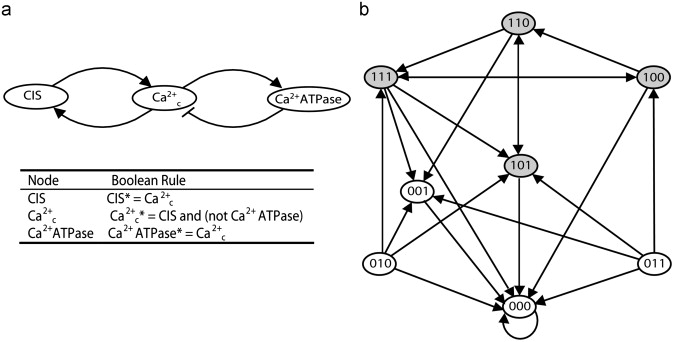
\includegraphics[width=0.9\linewidth]{gfx/red3nodos}
%\caption[Modelo Booleano de 3 nodos]{Modelo Booleano de 3 nodos de \citeauthor{Reka3Nodos2010} \citep{Reka3Nodos2010}.\ a) Reglas L\'ogicas.\ b) Estados posibles de la red.}\label{fig:red3reka}
%\end{figure}


%Si bien este modelo no está relacionado con la red de señalización discutida en esta tesis, el hecho de contar con pocos nodos sirvió como un buen punto de partida para transformar un modelo Booleano en uno de ecuaciones de Glass.

\section{Modelo discreto de la vía de señalización inducida por speract}\label{sect:erizo}


\citeauthor{Espinal2011} \citep{Espinal2011} presentan un modelo discreto en tiempo y estado para la vía de señalización inducida por speract en el flagelo del esperma de erizo de mar. En ese trabajo la red se compone de veintidós nodos, de los cuales  dieciocho toman valores de estado $0$ ó $1$, mientras que los cuatro nodos restantes tienen un valor de estado ternario, es decir, cada uno de estos nodos puede encontrarse en el estado $0$, $1$ ó $2$. Los nodos ternarios son los correspondientes al \acf{v}, \acf{ca}, \acf{hva} y \acf{lva}. Esta extensión a tres valores posibles es necesaria para capturar los estados posibles en los que se puede encontrar un componente de esta red de señalización. La figura \ref{fig:erizoModelo} muestra un diagrama de las conexiones de la misma vía de señalización presentada en la sección \ref{sec:spSigNet} e ilustrada en la figura \ref{fig:erizobBioquimica}. Los cuadros amarillos y verdes indican nodos binarios y ternarios, respectivamente. Las flechas negras indican activación, las líneas rojas inhibición y las flechas amarillas pueden representar activación o inhibición, dependiendo del valor del nodo correspondiente al \acf{v}. Los números sobre las flechas corresponden a las referencias con las que \citeauthor{Espinal2011} \citep{Espinal2011} construyeron la red y sustentan cada interacción. A manera de ejemplo, la función reguladora o tabla de verdad del nodo de \ac{cAMP} se muestra en la esquina inferior izquierda. Las primeras 3 columnas en esta tabla contienen todos los valores posibles de activación de los reguladores de \ac{cAMP}: \ac{AC}, \ac{pde} y \ac{cAMP}; la cuarta columna muestra los valores para la función que corresponden a cada combinación de los reguladores.

\begin{figure}[hbt]
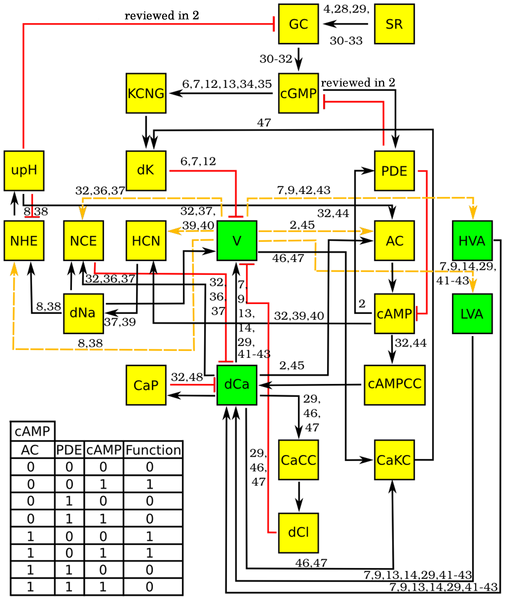
\includegraphics[width=0.9\linewidth,height=10cm]{gfx/redErizoModelo}
\caption[Modelo Discreto de la red de se\~nalizaci\'on]{Modelo Discreto de la red de se\~nalizaci\'on \citeauthor{Espinal2011} \citep{Espinal2011}. La figura muestra el diagrama de conexiones de la vía de señalización. Las flechas negras y rojas representan activación e inhibición, respectivamente. Las flechas naranjas son de activación o inhibición en función del valor del \acf{v}. Los números sobre las flechas corresponden a las referencias con las que \citeauthor{Espinal2011} \citep{Espinal2011} construyeron la red y sustentan cada interacción. En la parte inferior izquierda se muestra la tabla de la función de regulación para \ac{cAMP}.%Los cuadros amarillos y verdes indican nodos binarios y ternarios, respectivamente. Las flechas negras indican activación, las líneas rojas inhibición y las flechas amarillas pueden representar activación o inhibición, dependiendo del valor del nodo de voltaje $(V)$. A manera de ejemplo, la función reguladora o tabla de verdad del nodo de $cAMP$ se muestra en la esquina inferior izquierda. Las primeras 3 columnas en esta tabla contienen todos los valores posibles de activación de los reguladores de $cAMP$, $(AC,\ PDE,\ cAMP)$; la cuarta columna muestra los valores para la función que corresponden a cada combinación de los reguladores.
}\label{fig:erizoModelo}
\end{figure}

\begin{figure}[hbt]
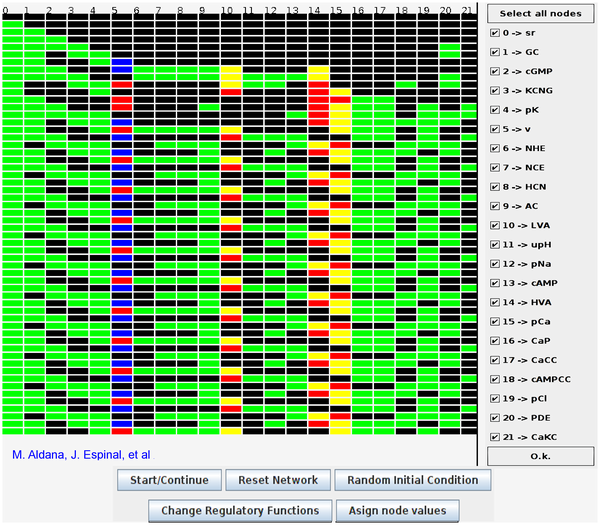
\includegraphics[width=0.9\linewidth%,height=10cm
]{gfx/appletErizo}
\caption[Applet del Modelo Discreto]{Applet del Modelo Discreto de la red de se\~nalizaci\'on \citeauthor{Espinal2011} \citep{Espinal2011}.\ Serie temporal de los patrones de activación de la red de señalización. Los nodos binarios se presentan en negro y verde, correspondientes a \emph{apagado}($0$) y \emph{encendido} ($1$). Los nodos ternarios correspondientes a los canales \ac{hva} y \ac{lva}, el negro es un estado inactivo ($0$), el amarillo ($1$) corresponde a un canal cerrado y el rojo ($2$) a un canal abierto. El nodo correspondiente al \acf{v} es negro ($0$) para un potencial en reposo, azul para la hiperpolarización ($1$) y rojo ($2$) para la repolarización. El nodo correspondiente al \ac{calintra} es amarillo ($1$) para indicar el incremento tónico, rojo ($2$) para el incremento supratónico y negro ($0$) para indicar estado basal. Se muestra el comportamiento del espécimen silvestre o \emph{wild type}.
El applet fue desarrollado por el Dr. Maximino Aldana y se encuentra disponible en \url{http://www.fis.unam.mx/research/seaurchin/discrete/}.}\label{fig:appletErizo}
\end{figure}

Para explorar distintas configuraciones iniciales, cambiar las reglas lógicas así como observar el comportamiento de la red en ausencia de algunos nodos, \citeauthor{Espinal2011} \citep{Espinal2011} presentan un \emph{applet} que permite explorar estas condiciones de manera interactiva. La figura \ref{fig:appletErizo} muestra una captura de pantalla de esta aplicación, donde se simula un organismo silvestre, es decir, una simulación en la que no se han realizado alteraciones a las reglas lógicas ni se han borrado nodos. Los nodos se presentan en el eje horizontal y el tiempo corre de arriba hacia abajo. Para los nodos binarios, el negro representa el estado \emph{apagado}, verde \emph{encendido}. Los nodos $10$ y $14$, correspondientes al \ac{hva} y \ac{lva}, el negro es un estado inactivo, el amarillo corresponde a un canal cerrado y el rojo a un canal abierto. El nodo 5, correspondiente al \acf{v} es negro para un potencial en reposo, azul para la hiperpolarización y rojo para la repolarización. El nodo 15 $(dCa)$, correspondiente al \ac{calintra} es amarillo para indicar el incremento tónico, rojo para el incremento supratónico y negro para indicar estado basal. Como puede observarse, bajo estas condiciones y para la condición inicial mostrada en la figura, tras un transitorio la red llega a un atractor de período 4.

\citeauthor{Espinal2011} \citep{Espinal2011} determinan que las configuraciones iniciales posibles para este modelo llegan a una de dos configuraciones cíclicas o atractores, uno de período cuatro y otro de período ocho. Estos atractores se relacionaron con las mediciones experimentales de fluorescencia de \ac{ca} en el flagelo del espermatozoide. Bajo el criterio de \citeauthor{huang2005} \citep{huang2005} mencionado en la sección anterior, los atractores del modelo discreto de la red de señalización de speract determinan las oscilaciones estables de \ac{ca} que posibilitan la relocalizaci\'on de los espermatozoides a trav\'es de las alteraciones que el \ac{ca} induce a la curvatura del flagelo. El 80\% de las configuraciones iniciales posibles convergen al atractor de período cuatro. El período cuatro de este atractor corresponde a una oscilación del tren de oscilaciones que se observa en las mediciones experimentales como la de la figura \ref{fig:fluorescencia} \citeauthor{Espinal2011} \citep{Espinal2011}.

Un paso fundamental al proponer un modelo para un sistema biológico consiste en comparar los resultados de dicho modelo con comportamientos que se hayan observado previamente mediante técnicas experimentales. A este proceso se le conoce como validación del modelo. El modelo presentado en \citeauthor{Espinal2011} \citep{Espinal2011} corrobora en un nivel cualitativo comportamientos observados experimentalmente, por ejemplo:
\begin{itemize}
\item En ausencia de speract, todas las condiciones iniciales alcanzan las condiciones basales tras un pequeño transitorio. De esta manera se confirma el papel que juega el speract para disparar las oscilaciones de \ac{calintra} \citeauthor{Espinal2011} \citep{Espinal2011}.
\item Si el nodo correspondiente a la \ac{dK} se elimina, las oscilaciones de \ac{calintra} se suprimen. Este comportamiento se ha observado experimentalmente en \citeauthor{Babcock:1992uf} \citep{Babcock:1992uf}.
\end{itemize}

\begin{figure}[hbt]
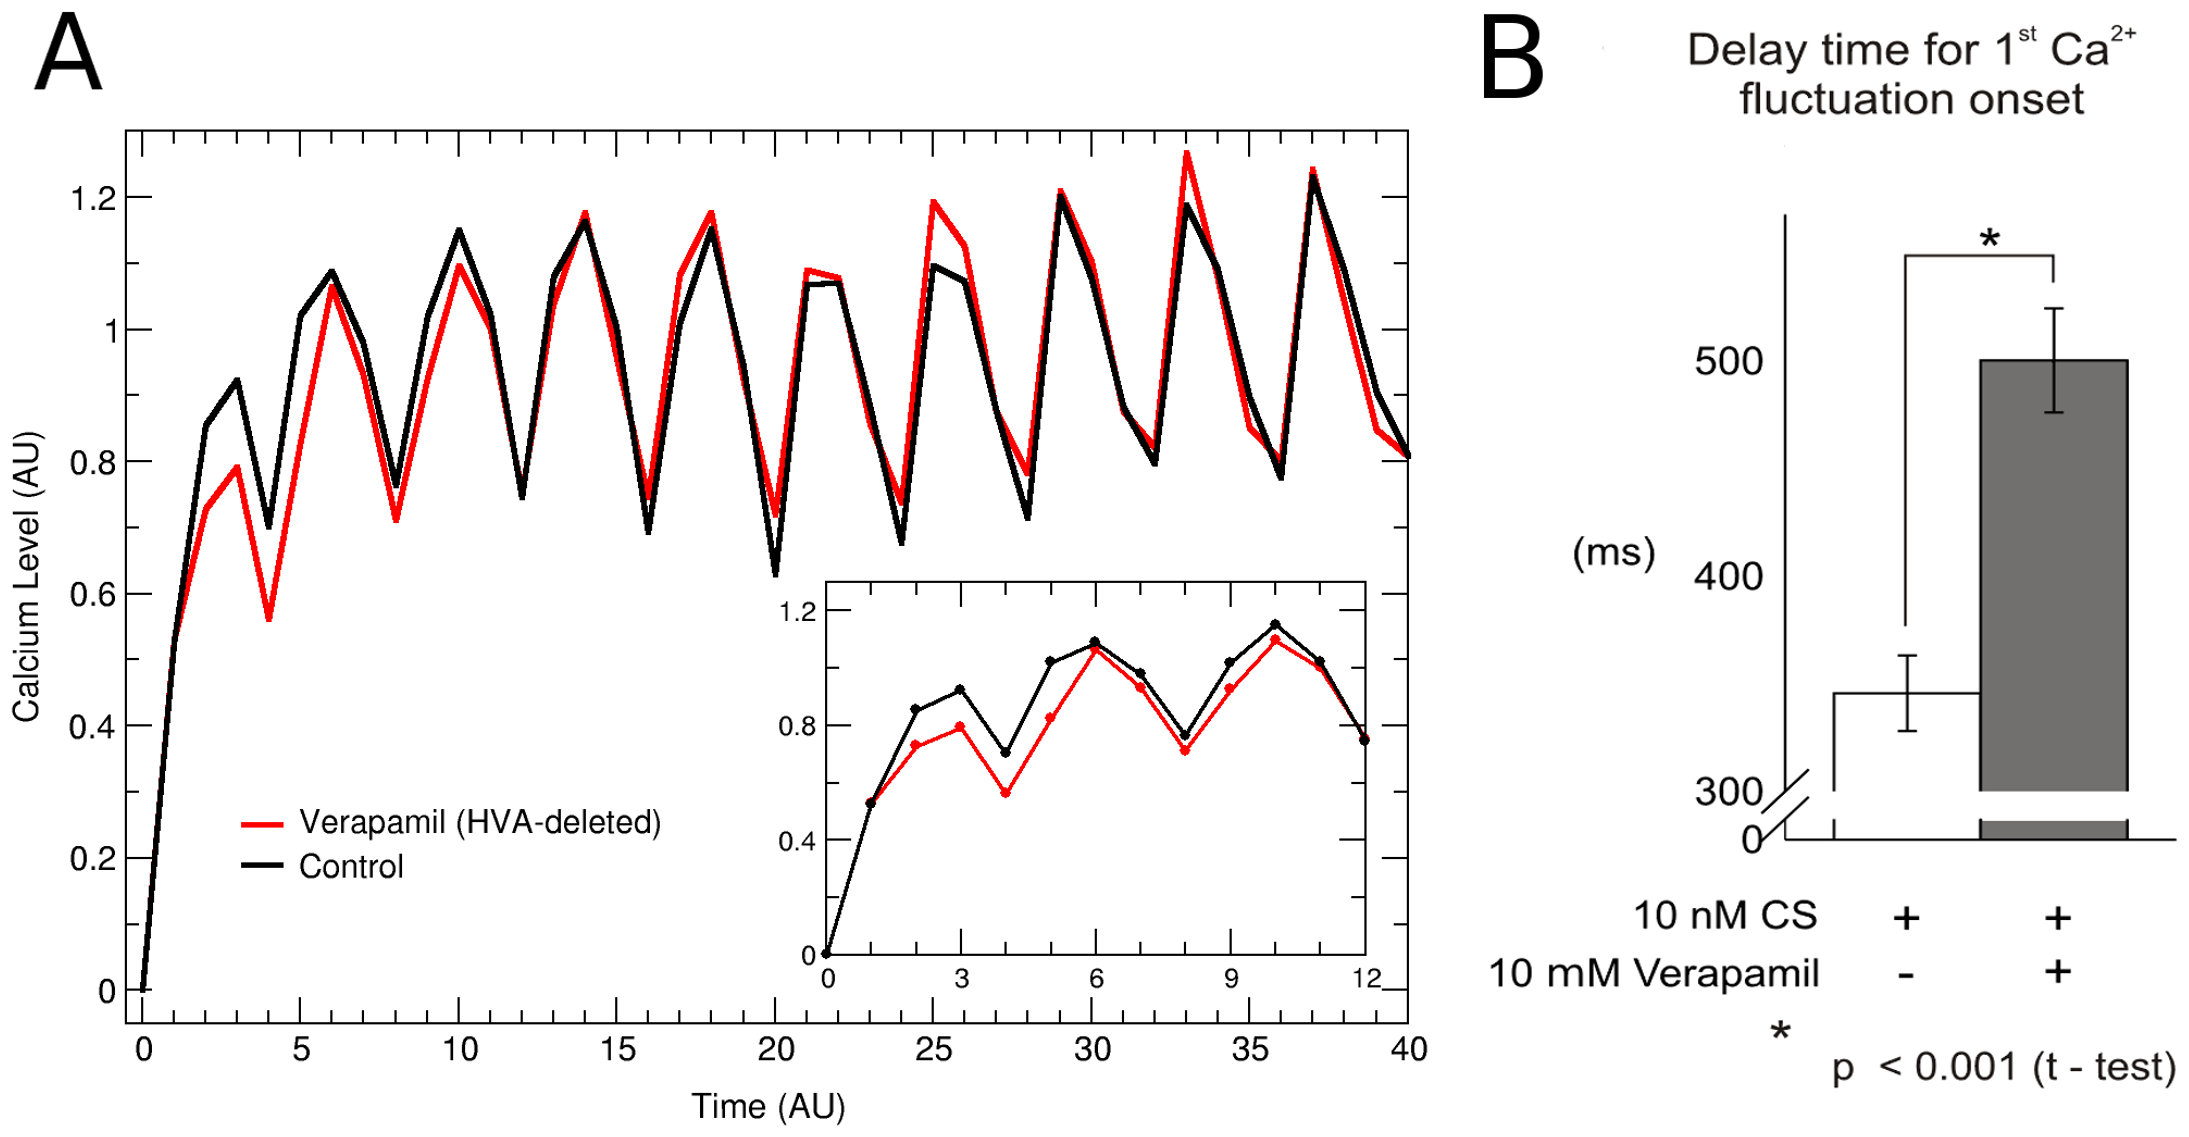
\includegraphics[width=0.9\linewidth]{gfx/figura8Chucho}
\caption[El bloqueo del canal \ac{hva} retrasa el inicio de las oscilaciones de \ac{ca}]{El bloqueo del canal \ac{hva} retrasa el inicio de las oscilaciones de \ac{ca}. A) Evolución temporal del nivel promedio de \ac{ca} tomado a cada paso de tiempo durante $10^5$ condiciones iniciales con \ac{hva} (curva negra) y sin \ac{hva} (curva roja), usando unidades arbitrarias. Nótese que cuando el canal \ac{hva} está presente el incremento en los niveles de \ac{ca} comienza más rápidamente que cuando se suprime el canal \ac{hva}, es decir, en los primeros pasos de tiempo, la curva negra se incrementa antes que la curva roja. La gráfica más pequeña es un acercamiento a los primeros pasos de tiempo de la dinámica. B) Los experimentos realizados muestran que el verapamil, sustancia que inhibe al canal \ac{hva}, prolonga el tiempo entre la estimulación de speract y el establecimiento de la primera fluctuación de \ac{ca}. \citeauthor{Espinal2011} \citep{Espinal2011}.}\label{fig:verapamil}
\end{figure}

El modelo de la vía de señalización de speract predijo dos comportamientos que no se habían observado experimentalmente. En particular, uno de ellos consiste en que al suprimir el canal \ac{hva}, aumenta el tiempo para que la concentración de \ac{ca} alcance los valores de alta intensidad que provoca la unión del speract a su receptor. Esta condición fue el comportamiento observado en promedio para $10^5$ condiciones iniciales diferentes. A raíz de este resultado del modelo se realizaron experimentos añadiendo $10  nm$ de \emph{verapamil}, un inhibidor del canal \ac{hva}. El bloqueo de este canal produce un retraso en la aparición de la primera fluctuación de \ac{calintra} en el flagelo del espermatozoide, lo cual valida a un nivel cualitativo la predicción hecha por el modelo. Este resultado se muestra en la figura \ref{fig:verapamil}

Como se puede observar en el apartado B de la figura \ref{fig:verapamil}, el tiempo medio para la aparición de la primera oscilación de \ac{ca} tras la adición de speract al medio es de alrededor de $500 ms$ en presencia de verapamil, en contraste con los $~350 ms$ del tipo silvestre. 

\section{Alcances y limitaciones del modelo discreto}

%% Este párrafo quedaría mejor en la justificación del modelo semicontinuo.
La figura \ref{fig:appletErizo} muestra que el modelo discreto divide una oscilación de \ac{ca} en cuatro subintervalos discretos en el tiempo. El valor discreto de un nodo cualquiera de la red en un subintervalo de tiempo, puede interpretarse como el promedio de los valores continuos que tomó ese nodo en el subintervalo: si dicho valor promedio fue mayor que un umbral, el estado discreto en todo el subintervalo es 1, y 0 en caso contrario. Lo que se quiere poner de manifiesto con esta observación es que las comparaciones entre un modelo discreto y las mediciones experimentales son a un nivel cualitativo y con una resolución temporal lo suficientemente grande como para contener en un paso de tiempo discreto varios cambios de estado continuo. Un modelo discreto es capaz de describir cómo cambia un sistema en una escala de tiempo más grande que aquella en la que suceden los eventos microscópicos del sistema. De ahí la necesidad de contar con otro tipo de descripciones del sistema que permitan hacer comparaciones entre modelo y experimentos en escalas de tiempo más pequeñas. Además, es deseable que dichas descripciones permitan hacer una comparación más precisa entre los valores de las variables de estado y las mediciones experimentales, por ejemplo, donde las variables de estado del modelo sean continuas.

Una de las limitaciones de dicho modelo consiste en que el sistema es sincronizado, es decir, todos los nodos actualizan su estado con el mismo esquema temporal. Esta actualización sincronizada es particularmente válida en tanto que el estado del nodo es un promedio en un intervalo de tiempo cuya duración es mayor que el tiempo en el que se dan las reacciones bioquímicas de la red. Sin embargo, aunque válido en algunos casos, el describir al sistema en intervalos de actualización largos es también una desventaja, puesto que no toma en cuenta la variedad de escalas temporales que presentan los distintos tipos de procesos biológicos, \citeauthor{Reka3Nodos2010} \citep{Reka3Nodos2010}. Como consecuencia de la escala temporal artificial de los modelos sincronizados, las comparaciones de éstos con experimentos solo pueden darse a un nivel cualitativo. Finalmente, la discretización de las variables de estado es adecuada para tener una idea general --no particular-- de la dinámica del sistema. 

\section{Ecuaciones de Glass}

Una opción de modelación intermedia entre los modelos discretos y los basados en las \ac{EDOs} son los de dinámica semicontinua. Entre este tipo de modelos se encuentran las ecuaciones lineales por pedazos que fueron esbozadas por Glass en \citeauthor{Glass1973} \citep{Glass1973}, consistentes en definir una derivada cuya forma específica depende del valor de un mapeo discreto en un intervalo de tiempo pequeño. En particular este mapeo puede ser una red Booleana como las presentadas en la sección \ref{boolNets}.

\subsection{Construcción de las ecuaciones de Glass}

Consideremos de nuevo el mapeo discreto \ref{eqn:kaufman}. Es posible escribirlo también como

\begin{equation}
\sigma_i(t+\tau_i)=F_i[\sigma_{i_1}(t),\sigma_{i_2}(t),\ldots,\sigma_{i_m}(t)]
\end{equation}
\\
donde $\tau_i=1$. Si $\tau_i \rightarrow 0$, haciendo un desarrollo en serie de Taylor de $\sigma_i(t+\tau_i)$ hasta la derivada de primer orden, para posteriormente despejar esa derivada se obtiene

\begin{equation}
\frac{d\sigma_i(t)}{dt} = \frac{1}{\tau_i} [\sigma_i(t+\tau_i) - \sigma_i(t)]
\end{equation}
\\
y sustituyendo $\sigma_i(t+\tau_i)$ por 

\begin{equation}
F_i[\hat{\sigma}_{i_1}(t), \hat{\sigma}_{i_2}(t), \ldots, \hat{\sigma}_{i_m}(t)]
%H(\sigma_{i_1}(t), \theta_{i_1}), H(\sigma_{i_2}(t), \theta_{i_2}),\ldots, H(\sigma_{i_k}(t), \theta_{i_k})]
\end{equation}
\\
donde

\begin{equation}
\hat{\sigma}_{i_j}(t) = H(\sigma_{i_j}(t), \theta_{i_j})\quad 1\le j \le m
\end{equation}
\\

obtenemos 

\begin{equation}
\frac{d\sigma_i(t)}{dt} = \frac{1}{\tau_i} (F_i[\hat{\sigma}_{i_1}(t), \hat{\sigma}_{i_2}(t), \ldots, \hat{\sigma}_{i_m}(t)]
 - \sigma_i(t))
\end{equation} 
\\
donde $\frac{1}{\tau_i}$ es el inverso del tamaño del intervalo donde se hace el desarrollo en serie de Taylor y $H(\sigma_{i_j}(t), \theta_{i_j})$ es una función escalón que discretiza los valores de estado del nodo $i_j$ al tiempo $t$ usando un valor de umbral $\theta_{i_j}$. Esta discretización es necesaria puesto que las variables de estado $\sigma_i$ son ahora variables continuas, al igual que el tiempo. Todos los $F_i$ son los mapeos del modelo discreto a partir del cual se construyeron las ecuaciones de Glass.

Mediante este procedimiento, es posible contar con una descripción semicontinua de la dinámica del sistema. La derivada de cada nodo no es única sino que depende del valor de la función discreta en cada intervalo de tamaño $\tau_i$. La derivada para un nodo Booleano es de la forma

\begin{equation}
\frac{d\sigma_i(t)}{dt} = \left\{
    \begin{array}{rr}
      \frac{1}{\tau_i} (1 - \sigma_i(t)) & \text{si } F_i[\hat{\sigma}_{i_1}(t), \hat{\sigma}_{i_2}(t), \ldots, \hat{\sigma}_{i_m}(t)] = 1\\
      \frac{1}{\tau_i} (0 - \sigma_i(t)) & \text{si } F_i[\hat{\sigma}_{i_1}(t), \hat{\sigma}_{i_2}(t), \ldots, \hat{\sigma}_{i_m}(t)] = 0
    \end{array} \right.
\end{equation} 
\\

A este tipo de ecuaciones se les conoce también como \emph{Piecewise Linear Differential Equations}, o Ecuaciones Diferenciales Lineales por Pedazos.
%% (Conviene tener una gráfica que ilustre por qué esto es realmente un mapeo piecewise linear, o de manera equivalente mostrar formalmente una de las ecuaciones diferenciales como un mapeo)

\subsection{Ventajas y desventajas}

El beneficio directo de usar el formalismo de las ecuaciones de Glass es contar con un refinamiento de las descripciones temporal y de estado que es capaz de producir un modelo discreto. Además, como se acaba de mostrar en su planteamiento, por construcción las ecuaciones de Glass incluyen un modelo discreto que a su vez fue planteado a partir de observaciones y conocimiento biológico. De este modo, estas ecuaciones semicontinuas no son un formalismo \emph{ad hoc} que reproduce el comportamiento de un sistema a través de ajustar arbitrariamente trayectorias, sino que se basan en un conjunto de observaciones y conocimiento previo.

El costo por usar este formalismo radica en la estimación de los valores de umbral para cada nodo de la red. En el caso de que se quiera un modelo sincronizado, los inversos de los tiempos característicos, que denotamos como $\alpha_i=\frac{1}{\tau_i}$ pueden establecerse todos iguales. En particular, el modelo discreto en tiempo se recupera al establecer el tiempo característico en $\tau_i = 1,\ \forall i$.

En este sentido, el problema de construir un modelo semicontinuo usando ecuaciones de Glass se reduce a un problema de estimación de parámetros. Estos parámetros son los umbrales de activación de cada nodo, además de los inversos del tamaño de cada uno de los intervalos de tiempo. Los parámetros deben elegirse de modo que la dinámica del sistema y de los nodos en particular sea coherente desde un punto de vista biológico.

\section{Estimación de parámetros}

La estimación de parámetros es un problema de optimización, consistente en encontrar parámetros tales que un modelo que dependa de ellos, minimice el error entre la solución al modelo y mediciones experimentales, es decir, que se \emph{ajuste} o \emph{explique} un conjunto de datos experimentales.

Para resolver un problema de optimización, es necesario definir una función, conocida como función objetivo, función de adaptación o función de costo, que permita asignar un valor a cada solución factible. Dependiendo de la manera en que esté definida, puede buscarse minimizar o maximizar la función objetivo. Los problemas de maximización y minimización son equivalentes, ya que minimizar una función $f$ es lo mismo que maximizar $h=-f$. Además de plantear una función para minimizar o maximizar, resulta útil contar con una estrategia de exploración del espacio de soluciones. 

De manera formal, sea $f(\mathbf{p})$ la función de costo a minimizar (o función de adaptación a maximizar), donde $f:\mathbb{R}^n\rightarrow \mathbb{R}$ y $\mathbf{p}$ es un vector de números reales. El valor de la función $f(\mathbf{p})$ indica la adaptación o costo del vector $\mathbf{p}$. Típicamente, en muchos problemas el gradiente de $f$ es desconocido. El objetivo consiste en encontrar $\mathbf{m} \in \mathbb{R}^n$ tal que $f(\mathbf{m}) \le f(\mathbf{p}),\ \forall \mathbf{p} \in \mathbb{R}^n$. En el caso de maximización, basta con definir la función $h=-f$. En este trabajo se optó por la minimización de funciones objetivo.

\subsection{Funciones de comparación}\label{ch1FuncComp}

Para el tipo de problemas de optimización discutidos en esta tesis, las funciones objetivo que se planteen, deben de permitir establecer una noción de distancia para determinar el grado de similitud entre una serie temporal proveniente de datos experimentales, y una serie temporal de la solución a un problema de condiciones iniciales de la ecuación de Glass correspondiente a dicha medición experimental.

Existen varias maneras de comparar series de tiempo, desde técnicas generales y ampliamente usadas como el \emph{Error Cuadrático Medio} \textsc{(mse)} \citep{msewiki}, el \emph{Coeficiente de Correlación de Pearson} \citep{pearsoncorrwiki}, hasta aquéllas que fueron diseñadas con el objetivo de establecer la similitud entre series de tiempo surgidas de procesos biológicos, como el \emph{Índice de Pendiente o Slope Index} \textsc{(si)} \citeauthor{Cho2006} \citep{Cho2006}.% Además se pueden usar algunos otros criterios que califiquen la similitud de dos trayectorias basados no solo en la distancia sino en propiedades específicas de un conjunto de parámetros que influyen sobre esa dinámica. En este último grupo se encuentra la \emph{Regularización Promotora de Dispersión o Sparsity Promoting Regularization} \citeauthor{Engl2009}.%(Van der Boos, Engels 2009, Vogel).

\subsubsection{Error Cuadrático Medio (MSE)}\label{MSE}

El \textsc{mse} \citep{msewiki} es el cuadrado del valor esperado de la diferencia entre las observaciones y la respuesta, trayectoria o dinámica predicha por un modelo. Al ser minimizado, es posible discriminar entre distintos modelos, estableciendo cuál de entre un conjunto de modelos ajusta mejor, es decir, explica mejor los datos. El \textsc{mse} está dado por 
\begin{equation}
E[(Y - X)^2]
\end{equation}
\\
donde $X$ son los datos experimentales, $Y$ son los datos del modelo que se quiere ajustar a dichos datos y $E$ es el valor esperado de la diferencia entre los conjuntos de datos $X$ y $Y$, es decir

\begin{equation}
	E = \frac{1}{n} (Y_i - X_i)^2
\end{equation}
\\
donde $X_i$ y $Y_i$ denotan las $i$ésimas mediciones de $X$ y $Y$, respectivamente y $n$ es el número de datos.



\subsubsection{Coeficiente de correlación de Pearson}\label{pearson}

El Coeficiente de Correlación de Pearson \citep{pearsoncorrwiki} es una medida de la correlación (dependencia lineal) entre dos variables aleatorias $X$ y $Y$, denotado por $r \in [-1, 1]$, está dado por
\begin{equation}\label{pearsonEQ} 
r_{\mathbf{X},\mathbf{Y}} = \frac{\sum_{i=1}^n (X_i - \bar{X})(Y_i - \bar{Y})} {\sqrt{\sum_{i=1}^n (X_i - \bar{X})^2} \sqrt{\sum_{i=1}^n (Y_i - \bar{Y})^2}}
\end{equation}
\\
donde $\bar{X}$ y $\bar{Y}$ son los promedios de $X$ y $Y$, respectivamente, $X_i$ y $Y_i$ denotan las $i$ésimas mediciones de $X$ y $Y$, respectivamente y $n$ es el número de datos. En este trabajo se identifica a los datos experimentales como $X$ y a $Y$ como los datos provenientes de la solución de un modelo (es decir, el modelo que se desea hacer coincidir con esos datos experimentales).

\subsubsection{Índice de Pendiente (SI)}\label{slopeIndex}

Propuesto por \citeauthor{Cho2006} \citep{Cho2006}, el índice de pendiente entre dos series de tiempo $X$ y $Y$ consiste en ponderar la suma de los signos de las derivadas entre los puntos de ambas series. Está dado por 

\begin{equation}\label{siEQ}
SI(X,Y) = \frac{1}{n - 1} \sum_{i=1}^{n-1} \mathtt{signo} \left(\frac{X_{i+1} - X_i} {Y_{i+1} - Y_i}\right)
\end{equation}
\\
donde $X_i$ y $Y_i$ denotan las $i$ésimas mediciones experimental de $X$ y $Y$, respectivamente, $n$ es el total de mediciones experimentales y signo es una función  definida como $\mathtt{signo}: \mathbb{R} \rightarrow \{ -1,0,1 \} $ dada por
\begin{equation*}
  \mathtt{signo}(a) = \left\{
    \begin{array}{rl}
      -1 & \text{si } a < 0,\\
      0 & \text{si } a = 0,\\
      1 & \text{si } a > 0.
    \end{array} \right.
\end{equation*}
\\
Se excluyen aquellos puntos en los cuales $Y_{i+1} - Y_i = 0$. De manera similar al coeficiente de correlación de Pearson, $SI(X,Y)\in [-1, 1]$, $X$ representa a los datos experimentales y $Y$ los datos provenientes de la solución de un modelo (es decir, el modelo que se desea hacer coincidir con esos datos experimentales).

\subsection{Estrategias de exploración}

Una vez que se tiene definida una función objetivo o función de costo que permita evaluar las distintas soluciones factibles al problema, es necesario contar con una estrategia de búsqueda o exploración que permita explorar el espacio de soluciones factibles. Además, es deseable que la estrategia de búsqueda explore de manera inteligente el espacio de soluciones, es decir, que evite que la búsqueda quede atrapada en puntos extremos locales y que por ende sea imposible encontrar los puntos extremos globales.

\subsubsection{Tipos de exploración}

Además de la búsqueda al azar, existen dos estrategias generales para resolver problemas de optimización: aquéllas basadas en la diferenciabilidad de la función de costo, y aquéllas basadas en el uso de criterios heurísticos.
Un ejemplo clásico de un método basado en diferenciabilidad es el de Gradiente Conjugado, \citeauthor{numrecipesc} \citep{numrecipesc}. Entre los métodos populares basados en criterios heurísticos se encuentran el \textsc{Recocido Simulado}, \citeauthor{Kirkpatrick1983} \citep{Kirkpatrick1983}, y los \textsc{Algoritmos Genéticos}, \citeauthor{Goldberg1989} \citep{Goldberg1989}.

Las métodos basados en diferenciabilidad suelen usarse cuando se conoce con un buen nivel de detalle el espacio de soluciones, y en ese caso permiten encontrar los puntos extremos globales fácilmente. Sin embargo, una mala elección del punto inicial de búsqueda puede resultar en que estos algoritmos de optimización queden atrapados en un punto extremo local. Hacer malas elecciones del punto inicial de búsqueda suele ser común cuando no se conoce muy a fondo el espacio de soluciones. Por ello, estos métodos son útiles para refinar soluciones, es decir, para aumentar la precisión de una solución una vez que se cree que se está cerca de un punto extremo global, o al menos, cerca de un punto cuyo valor es cercano al punto extremo global.

Por otro lado, los métodos de búsqueda basados en criterios heurísticos explotan propiedades del problema que no necesariamente están relacionadas con la diferenciabilidad de la función objetivo o función de costo. Además, se ha observado que son más resistentes a quedar atrapados en puntos extremos locales, debido a que incluyen un subprocedimiento que permite variar de una u otra forma las soluciones propuestas, independientemente de si esta solución mejora o no el costo de la función objetivo. Por lo tanto, estos métodos no son tan sensibles a una mala elección del punto o puntos iniciales de búsqueda, y no es necesario conocer la forma específica del espacio de soluciones, \citeauthor{BangaMoles2003} \citep{BangaMoles2003}, \citeauthor{Storn1997} \citep{Storn1997}.

\section{Justificación y objetivo}

Tal y como se mostró en el experimento de bloqueo de \ac{hva}, el tipo de comparaciones que se pueden hacer entre el modelo discreto y los experimentos son a un nivel cualitativo. A pesar de que aún a este nivel es posible ganar entendimiento de la vía de señalización, el contar con un modelo más detallado en tiempo y estado sería útil para hacer comparaciones a nivel cuantitativo.
Adicionalmente, hay que considerar que al hacer más pequeño el tiempo en el que se actualiza el estado de un componente de la red, la asincronía, es decir, que cada componente o nodo de la red actualice su estado de acuerdo a su propio tiempo característico de reacción, se vuelve más relevante, \citeauthor{Reka3Nodos2010} \citep{Reka3Nodos2010}.

Una opción para refinar el modelo es plantear ecuaciones diferenciales ordinarias. Sin embargo, para esto se requiere conocer un conjunto de parámetros relacionados directamente con magnitudes físicas y bioquímicas, a saber: las concentraciones de cada componente de la vía de señalización; las tasas de asociación y disociación de cada complejo bioquímico, y finalmente, la cooperatividad de las reacciones bioquímicas, es decir, la cantidad de moléculas necesarias de un compuesto para que este reaccione con otro. Por lo general, estos parámetros no son conocidos en su totalidad y su estimación experimental es costosa, complicada desde el punto de vista de diseño y ejecución del experimento, o ambas. En el caso particular de esta red de señalización, no todos estos parámetros e información son conocidos, por lo que como primera aproximación se desarrolló el modelo discreto antes mencionado.

Un modelo basado en las ecuaciones de Glass es un tipo de descripción del sistema a un nivel de detalle que se encuentra entre una aproximación discreta y una continua como la proporcionada por un modelo basado en ecuaciones diferenciales ordinarias.

Es importante recalcar que las ecuaciones de Glass no son en modo alguno una alternativa excluyente del modelado que se pueda hacer con ecuaciones diferenciales ordinarias. Por el contrario, si bien es cierto que los parámetros temporales y de umbral de las ecuaciones de Glass no son los mismos parámetros cinéticos y de reacción que aparecen en los modelos basados en \ac{EDOs}, conocer los parámetros de las ecuaciones de Glass puede dar una idea cualitativa de la magnitud de los parámetros cinéticos. Este conocimiento cualitativo resultaría de gran utilidad al momento de querer plantear un sistema de ecuaciones diferenciales acopladas para la vía de señalización de speract.

El objetivo de este trabajo es mejorar, mediante el uso de ecuaciones de Glass, la descripción temporal y de estado de la vía de señalización que la proporcionada por el modelo discreto de \citeauthor{Espinal2011} \citep{Espinal2011}. 

Algunas de las funciones de regulación del modelo de \citeauthor{Espinal2011} \citep{Espinal2011}, en particular las correspondientes a los nodos de \ac{ca} y potencial de membrana, son bastante más complejas que las que aparecen en otros modelos discretos, por ejemplo el de diferenciación de la flor de la planta modelo  \emph{Arabidopsis thaliana} que presentan \citeauthor{EspinosaSoto:2004jr} \citep{EspinosaSoto:2004jr} y \citeauthor{AlvarezBuylla:2008cg} \citep{AlvarezBuylla:2008cg}, o el de diferenciación en el nicho de células madre de la misma planta desarrollado en \citeauthor{Azpeitia:2010ik} \citep{Azpeitia:2010ik}. En estos modelos, todos los nodos y por ende las funciones de regulación son estrictamente binarios, en contraste con los valores ternarios de los nodos de \ac{ca} y potencial de membrana y algunos de los reguladores de éstos en el modelo de \citeauthor{Espinal2011}. Por ello, se determinó que sería conveniente ganar entendimiento del proceso de traducción de un modelo discreto en uno basado en ecuaciones de Glass, ayudándose de un modelo discreto con una dinámica más sencilla. En particular, dentro de  \citeauthor{Reka3Nodos2010} \citep{Reka3Nodos2010} se presenta una red discreta pequeña de tres nodos, donde los valores de estado son estrictamente Booleanos. La elección de esta red se basa solo en su simplicidad, a la par de que no es una red artificial sino una subred de una vía de señalización en plantas. Los modelos que se presentan en \citeauthor{EspinosaSoto:2004jr} \citep{EspinosaSoto:2004jr}, \citeauthor{AlvarezBuylla:2008cg} \citep{AlvarezBuylla:2008cg} y \citeauthor{Azpeitia:2010ik} \citep{Azpeitia:2010ik} son bastante más complejos que esa red de tres nodos. La red de tres nodos se describe brevemente en el apéndice \ref{ch:3Nodos}.

\section{Resumen}
Este capítulo introdujo la vía de señalización de speract, que se ha relacionado con la motilidad del espermatozoide de erizo de mar. Mostró también un modelo discreto para esta vía de señalización, resaltando sus alcances y limitaciones. Introdujo el formalismo semicontinuo de las ecuaciones de Glass y mostró algunos aspectos relevantes para la construcción de un modelo de este tipo a partir de uno discreto. Además, se mencionó que el objetivo de esta tesis es desarrollar un modelo de ecuaciones de Glass para la vía de señalización de speract, y que para ganar entendimiento de este proceso, se desarrolló también un modelo semicontinuo para una red simple de tres nodos.

El siguiente capítulo aborda detalles necesarios para la construcción de los programas de ajuste de parámetros para ambos modelos de ecuaciones de Glass.

%Dado que las mediciones experimentales arrojan datos continuos tomados con una frecuencia bastante mayor que la descripción del modelo discreto, la comparación entre dicho modelo y las mediciones experimentales se puede hacer hasta un nivel de detalle limitado. Sería deseable contar con un modelo que pudiera dar una descripción continua en tiempo y estado, además de incorporar asincronía, es decir, que cada componente o nodo de la red actualice su estado de acuerdo a su propio tiempo característico de reacción. Para este fin bien podría plantearse un modelo basado en \textsc{EDOs}. Sin embargo, para hacerlo sería necesario conocer un conjunto de parámetros relacionados directamente con magnitudes físicas y bioquímicas, a saber: las concentraciones de cada componente de la vía de señalización; las tasas de asociación y disociación de cada complejo bioquímico, y finalmente, la cooperatividad de las reacciones bioquímicas, es decir, la cantidad de moléculas necesarias de un compuesto para que este reaccione con otro. Sin embargo, por lo general estos parámetros no son conocidos en su totalidad y su estimación experimental es costosa, complicada desde el punto de vista de diseño y ejecución del experimento, o ambas. Si bien se puede hacer la estimación de algunos de estos parámetros a través de modelos computacionales y de optimización, se requiere de cierto conocimiento previo del sistema para poder llevar a cabo la estimación de manera más dirigida y reducir el espacio de búsqueda.

%En el caso particular de esta red de señalización, no todos estos parámetros e información son conocidos, por lo que como primera aproximacion se desarrolló el modelo discreto antes mencionado. Un modelo basado en las ecuaciones de Glass constituye un refinamiento a la descripción del sistema proporcionada por el modelo discreto.